\documentclass{hw}
\usepackage[version=3]{mhchem}
\usepackage{nuc}
\usepackage{array}
\graphicspath{ {images/}}
\newcolumntype{L}{>{$}l<{$}}

\author{J.R. Powers-Luhn}
\date{2016/09/08}
\title{Homework \#3}

\begin{document}

\problem{}
	Calculate the geometric cross sections for $ \He{4} $ nuclei striking $ \ce{H} $ and $ \C{12} $. Using these cross sections, determine the geometric cross section for $ \ce{^4He + CH_2} $.

\solution 
	\begin{align*}
		\sigma &= \pi \left( R_1 + R_2 \right)^2 \\
		&= \pi \left( R_{\ce{^{4}He}} + R_{\ce{^{12}C}} \right)^2 \\
		R= r_0 A^{1/3} \\
		r_0 = 1.4*10^{-13}cm \\
		\intertext{First $ \ce{^{12}C} $:}
		\sigma_C &= \pi r_0^2 \left( 4^{1/3} + 12^{1/3} \right)^2 \\
		\sigma_C &= 0.925b
		\intertext{Next $ \ce{H} $:}
		\sigma_H &= \pi r_0^2 \left( 4^{1/3} + 1^{1/3} \right)^2 \\
		\sigma_H &= 0.412b
		\intertext{Finally we add them according to their number percentages:}
		\sigma_{\ce{CH_{2}}} &= 2 \sigma_H + \sigma_C \\
		\sigma_{\ce{CH_{2}}} &= 1.75b
	\end{align*}


\problem{}
	Compare the differences in stopping power determined from the two equations below for protons at 10, 100, and 500 MeV in aluminum.
		\begin{align}
			S_c &= 4 \pi r_0^2 m_e c^2 \left( \frac{z^2}{\beta^2} \right) \left( \frac{N_A \rho}{M_m} \right) Z \left( ln \left( \frac{2 m_e c^2 \gamma^2 \beta^2}{I} \right) - \beta^2 \right) \label{betablockwithbeta} \\
			S_c &= 4 \pi r_0^2 m_e c^2 \left( \frac{z^2}{\beta^2} \right) \left( \frac{N_A \rho}{M_m} \right) Z \left( ln \left( \frac{2 m_e c^2 \gamma^2 \beta^2}{I} \right)\right) \label{betablockwithoutbeta}
		\end{align}

\solution
	Constants:
	\begin{table}[h]
		\begin{tabular}{  L L  }
			r_0 & 2.8179*10^{-13}cm \\
			m_e & 0.511MeV \\
			c & 1 \\
			z & 1 \\
			N_A & 6.022*10^{23} \\
			\rho & 2.7 g/cm^3 \\
			M_m & 26.9815g/mol \\
			Z & 13 \\
			I & 162 eV
		\end{tabular}
	\end{table}

	Calculations are performed in the attached python notebook. Results:
	\begin{table}[h]
		\begin{tabular}{ |c|c|c| }
			\hline
			T (MeV) & Classical (MeV/cm) & Relativistic (MeV/cm) \\
			\hline
			10 & 93.3 & 92.9 \\
			100 & 15.8 & 15.4 \\
			500 & 6.29 & 5.89 \\
			\hline
		\end{tabular}
	\end{table}

	These disagree with PSTAR by factors in the approximate range of 3-4


\problem{}
	A point source of a radioisotope moves along a straight line past an observer (see diagram below). The distance of closest approach between the source and observer is equal to L. The dose rate at the distance of closest approach is known and has a value of $ \dot{D}_L $. If the source moves with a velocity $ v $, what is the total integrated dose at the observation point? Hint: see class notes on the derivation of the stopping power eqn.

	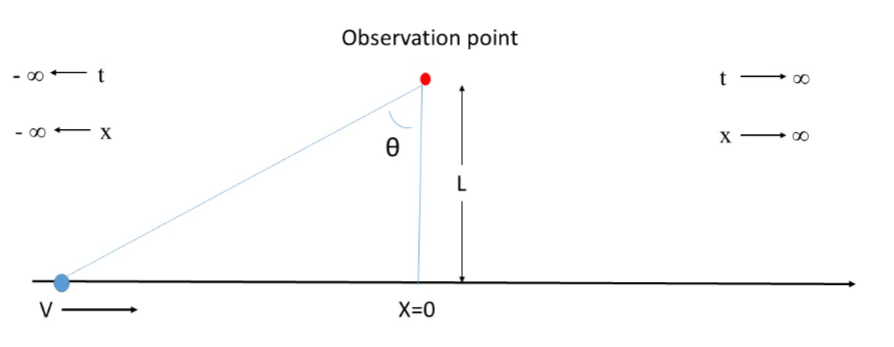
\includegraphics[width=15cm,height=10cm,keepaspectratio]{ne551_03_fig_01}

\solution
\[
	\dot{D}(r) = \dot{D_L}\frac{L^2}{r^2}
\]
	\begin{align*}
		r^2 &= x^2 + L^2 \\
		&= \left( vt \right)^2 + L^2
	\end{align*}

	We then intergrate over time:

	\begin{align*}
		D &= \int^{\inf}_{-\inf} \frac{\dot{D}_L L^2}{v^2 t^2 + L^2} dt \\
		&= \frac{\pi L \dot{D}_L}{v}
	\end{align*}

\problem{Anderson 2.5}
	\begin{enumerate}
		\item (Anderson 2.4) Calculate the rate of energy loss of a $ 2.5 MeV $ proton in aluminum. Use Equations 2.26 and 2.27 with no shell corrections or density corrections. Use the $ I_a $ value from Table 2.3.
		\item (Anderson 2.5) Amend the calculations of problem 4 by adding the shell correction and the effective charge correction.
	\end{enumerate}

\solution
	We compare the values produced by equation \ref{betablockwithoutbeta} and \ref{betablockwithbeta}, with \ref{betablockwithbeta} corrected in the log term with a value from Anderson fig 2.11.

	$ \delta = 0.19 $

	Producing:

	\[
	S_c = 4 \pi r_0^2 m_e c^2 \left( \frac{z^2}{\beta^2} \right) \left( \frac{N_A \rho}{M_m} \right) Z \left( ln \left( \frac{2 m_e c^2 \gamma^2 \beta^2}{I} \right) - \beta^2 - \delta \right)
	\]

	Calculations are performed in the attached program. The values produced are: 

	No corrections:

	$ S_c = 264.19 MeV/cm $

	With corrections applied:

	$ S_c = 256.26 MeV/cm $

\end{document}